\begin{figure}[!t]
    \centering
    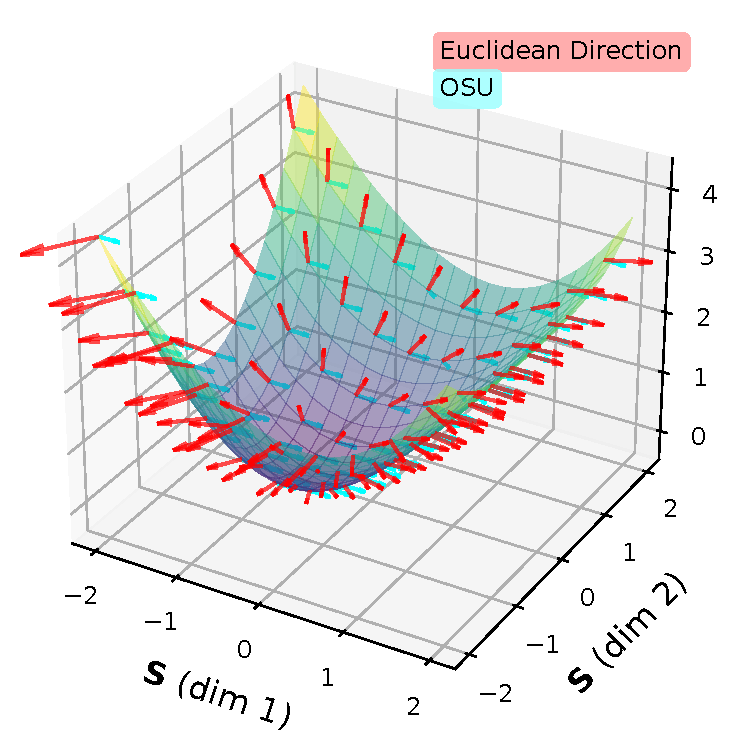
\includegraphics[width=0.98\linewidth]{fig/landscape/fig_landscape.pdf}
    \caption{\textbf{3D geometric intuition} of update directions on the loss landscape.
    The \hlred{Euclidean Direction} updates the state element-wise along the steepest descent, often ignoring local curvature.
    \hlcyan{OSU} evolves the state by projecting gradients via the matrix sign function, thereby maintaining the consistency of the underlying subspace structure.
    The $x$ and $y$ axes represent the two dimensions of the state $\mathbf{S}$.
    The movement toward the lower regions of the surface represents the direction of loss optimization.}
    \label{fig:landscape_3d_geo}
\end{figure}